\documentclass[12pt,titlepage,a4paper]{article}
\usepackage[utf8]{inputenc}
\usepackage[russian]{babel}
\usepackage{graphicx}
\usepackage[labelsep=period]{caption}
\textwidth=18cm
\oddsidemargin=-1.04cm
\headheight=0cm
\headsep=0cm
\topmargin=-1.04cm
\flushbottom
\setlength{\textheight}{51\baselineskip}
\setlength{\textheight}{\baselinestretch\textheight}
\addtolength{\textheight}{\topskip}

\begin{document}

\begin{titlepage}

\begin{center}
\large $\phantom{dirty trick}$

\vspace{0.2cm}

Министерство образования и науки Российской Федерации\\

\vspace{0.5cm}

Федеральное государственное автономное образовательное учреждение высшего образования

\vspace{0.5cm}

САНКТ-ПЕТЕРБУРГСКИЙ НАЦИОНАЛЬНЫЙ ИССЛЕДОВАТЕЛЬСКИЙ\\
УНИВЕРСИТЕТ ИНФОРМАЦИОННЫХ ТЕХНОЛОГИЙ,\\
МЕХАНИКИ И ОПТИКИ

\vspace{2.5cm}

Кафедра систем управления и информатики

\vspace{3.0cm}

Отчет по лабораторной работе~№1\\

\vspace{0.2cm}

<<ПОСТРОЕНИЕ МАТЕМАТИЧЕСКОЙ МОДЕЛИ ДВИГАТЕЛЯ NXT>>\\

\vspace{0.2cm}

по дисциплине <<Введение в специальность>>

\end{center}

\vspace{2.5cm}

{\large 
\begin{tabbing}
\hspace{12.5cm}\=\hspace{0.3cm}\=\+\kill
Выполнили:\'\>студенты гр.~P31**\+\\
Иванов~И.\,И.\\
Петров~П.\,П.\\
Сидоров~С.\,С.\-\\[\medskipamount]
Преподаватель:\'\>Капитонов~А.\,А.,\+\\
ассистент каф.~СУиИ
\end{tabbing}

}
\vspace{\fill}

\begin{center}
\large
Санкт-Петербург\\2016
\end{center}
\end{titlepage}

\addtocounter{page}{1}

\section{Цель работы}
\hspace{\parindent}Экспериментально проверить справедливость функций, описывающих работу ненагруженного двигателя постоянного тока, определить значение параметра $T_m$ последнего и, пользуясь результатами проделанных вычислений, проанализировать характер зависимостей $T_m(voltage)$ и $\omega_{nls}(voltage)$.

\section{Материалы работы}
\subsection{Результаты необходимых расчетов и построений}
\hspace{\parindent}Результаты аппроксимации экспериментальных данных соответствующей функцией от времени в виде значений величин $T_m$ и $\omega_{nls}$ сведены в таблицу~\ref{table:table_with_results}.
В~четвертом ее столбце указаны результаты расчета величины $M_{st}$ по значениям величин $T_m$ и $\omega_{nls}$  из двух предшествующих столбцов.

\begin{table}[h]
	\caption{Результаты расчетов величин $T_m$, $\omega_{nls}$ и $M_{st}$.}
	\centering\begin{tabular}{|c|c|c|c|}
	\hline
	$Voltage$, \% & $\omega_{nls}$, рад\slash с & $T_m$, с & $M_{st}$, Н$\cdot$м\\
	\hline
	100 & 16.423 & 0.091 & 0.415\\
	\hline
	80  & 13.197 & 0.087 & 0.349\\
	\vdots & \vdots & \vdots & \vdots\\
	-100 & -16.370 & 0.079 & 0.476\\
	\hline
	\end{tabular}
	\label{table:table_with_results}
\end{table}

\begin{figure}[h]
	\noindent\centering{
		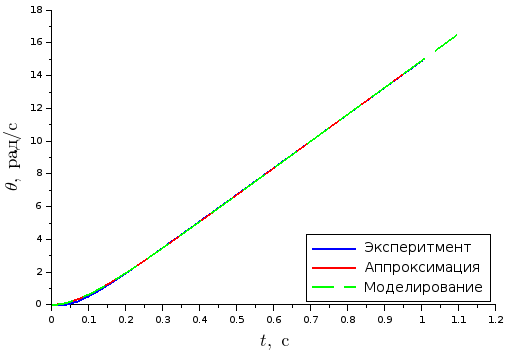
\includegraphics[scale=0.9]{100.png}
	}
	\caption{Графики зависимости угла поворота ротора от времени при $voltage=100$.}
\end{figure} 
\pagebreak
\begin{figure}[h]
	\noindent\centering{
		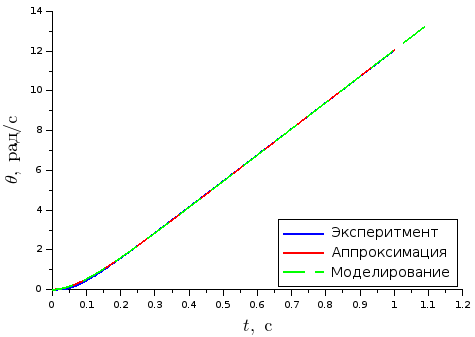
\includegraphics[scale=0.9]{80.png}
	}
	\caption{Графики зависимости угла поворота ротора от времени при $voltage=80$.}
\end{figure}
\addtocounter{figure}{7}
\begin{center}
\itshape Здесь, подразумевается, находятся еще 7 необходимых графиков.
\end{center}
\begin{figure}[h]
	\noindent\centering{
		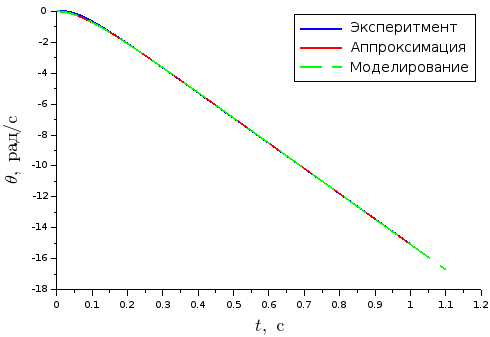
\includegraphics[scale=0.9]{m100.png}
	}
	\caption{Графики зависимости угла поворота ротора от времени при $voltage=-100$.}
\end{figure}
\pagebreak
\begin{figure}[h]
	\noindent\centering{
		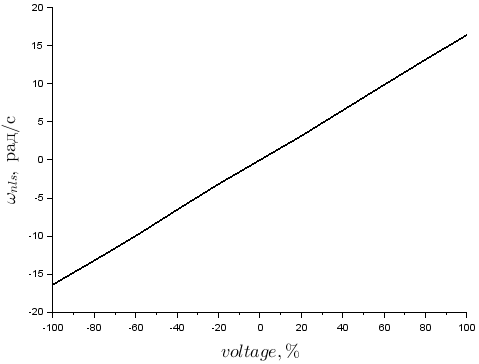
\includegraphics[scale=0.95]{omega_nls_power.png}
	}
	\caption{График зависимости $\omega_{nls}(voltage)$.}
\end{figure}
\begin{figure}[h!]
	\noindent\centering{
		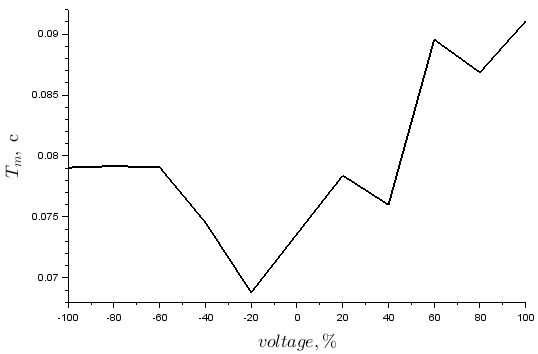
\includegraphics[scale=0.95]{Tm_power.png}
	}
	\caption{График зависимости $T_m(voltage)$.}
\end{figure}
\pagebreak
\subsection{Схема моделирования}
\begin{figure}[h]
	\noindent\centering{
		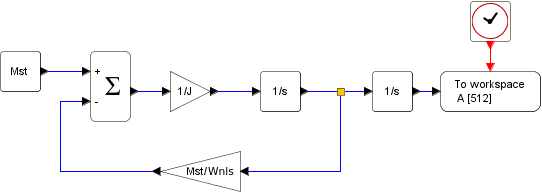
\includegraphics[scale=1.0]{struct_sheme_white.png}
	}
	\caption{Схема моделирования процесса разгона ненагруженного двигателя постоянного тока.}
\end{figure}


\subsection{Код основной расчетной программы}
\begin{verbatim}
    results=read("C:\for_scilab\my100.txt",-1,2);
    qlines=size(results,1);
    angle=results(:,1)
    angle=angle*%pi/180
    time=results(:,2)/1000
    plot2d(time, angle, 2)
    ...
\end{verbatim}
\subsection{Код программы для NXT}
\begin{verbatim}
    #define PERCENTS 60
    #define MOTOR_PORT OUT_B

    task main(){

         byte handle;
         int str_size;
         ...
         OnFwd(MOTOR_PORT, PERCENTS);
         first_time = CurrentTick();
         ...
         CloseFile(handle);
    }
\end{verbatim}
\section{Выводы}
\hspace{\parindent}В~результате проделанной работы было \dots
\begin{quote}
\itshape В~данном разделе требуется своими словами
\begin{itemize}
\item указать на то, что в работе было сделано все, что предписывалось выполнить заданием;
\item лаконично описать полученные результаты: результаты проверок, расчетов и т.д.~--- и прокомментировать их;
\item упомянуть о чем--либо ином, относящемся к работе, если это, на ваш взгляд, необходимо.
\end{itemize}
К~примеру в выводе отчета по первой работе логично отметить следующее:
\begin{itemize}
\item насколько кривые разгона двигателя (построенная по экспериментальным данным, построенная в соответствии с теоретически выведенным выражением и построенная по числовым значениям, полученным в результате моделирования соответствующей схемы в Xcos) совпадают друг с другом;
\item описать характер получившихся графиков для зависимостей $T_m(voltage)$ и $\omega_{nls}(voltage)$ и прокомментировать такой их вид.
\end{itemize}
\end{quote}
\end{document}